\chapter{Contesto aziendale}
\label{cap:azienda}

\intro{In questo capitolo viene descritto il contesto in cui l'azienda opera e come essa si approccia ai propri progetti.}

\section{Prodotti e servizi}

L'azienda si occupa di fornire servizi di consulenza, progettazione e sviluppo di soluzioni software e hardware, oltre a fornire servizi di \emph{outsourcing} dell'infrastruttura. Tra i clienti di Wintech possiamo trovare professionisti, PMI e grandi aziende, banche, assicurazioni e pubblica amministrazione.

I prodotti principali e più richiesti sono software per la gestione documentale e l'ottimizzazione dei processi aziendali, programmi \emph{ERP} e di \emph{Business Intelligence}, fino ad arrivare a consulenze personalizzate per soluzioni \emph{IT}, di \emph{CyberSecurity} e \emph{design} di \emph{intranet} aziendali.

\subsection{Cloud}
\label{sez:azienda-cloud}
Wintech offre servizi \emph{cloud} mirati alle aziende e certificati secondo lo standard ISO 27001. Per un cliente, questo si traduce nela possibilità di accedere a potenti risorse informatiche, affidabili e scalabili, senza dover effettuare grandi investimenti in una infrastruttura interna, con relativi costi di creazione, gestione e formazione dei dipendenti. Affidandosi quindi ad un fornitore con esperienza si può lavorare con la sicurezza di avere le ultime tecnologie senza doversi preoccupare dei rischi.\cite{site:wtc-cloud}

L'infrastruttura offerta da Wintech sfrutta strumenti all'avanguardia e si affida a partner nazionali di rilievo come \emph{VSIX} e \emph{DATA4} e internazionali quali \emph{Microsoft Azure} e \emph{Amazon AWS} (\autoref{fig:partner-cloud})

\begin{figure}[htbp]
    \centering
    \begin{subfigure}[b]{0.4\linewidth}
        \centering
        
\includegraphics[width=\linewidth]{images/loghi/vsix.png}
        \caption{Logo di VSIX}
        \label{fig:logo-vsix}
    \end{subfigure}
    \hfill
    \begin{subfigure}[b]{0.4\linewidth}
        \centering
        
\includegraphics[width=0.6\linewidth]{images/loghi/data4.png}
        \caption{Logo di DATA4}
        \label{fig:logo-data4}
    \end{subfigure}
    \hfill
    \begin{subfigure}[b]{0.4\linewidth}
        \centering
        
\includegraphics[width=\linewidth]{images/loghi/azure.png}
        \caption{Logo di Microsoft Azure}
        \label{fig:logo-azure}
    \end{subfigure}
    \hfill
    \begin{subfigure}[b]{0.4\linewidth}
        \centering
        
\includegraphics[width=0.8\linewidth]{images/loghi/aws.png}
        \caption{Logo di Amazon AWS}
        \label{fig:logo-aws}
    \end{subfigure}
    \caption{Loghi partner cloud di Wintech}
    \label{fig:partner-cloud}
\end{figure}

\subsection{Security}
\label{sez:azienda-security}

Negli ultimi anni l'ambito della sicurezza informatica per le aziende sta diventando sempre più di rilievo e di fondamentale importanza. Wintech si mantiene aggiornata in questo settore estremamente dinamico, dove ogni giorno vengono scoperte nuove falle e vulnerabilità, che devono essere tempestivamente risolte.

L'approccio di Wintech è quello di fornire soluzioni di sicurezza che siano in grado di proteggere i dati e le informazioni aziendali, definendo vari livelli di sicurezza per ogni tipo di risorsa. Tutte le soluzioni proposte dall'azienda sono costruite in modo da essere conformi al \emph{GDPR}, senza demonizzarlo, ma anzi andando a sfruttare le opportunità che esso offre per migliorare la sicurezza e la consapevolezza dei clienti.

In \autoref{fig:sec-matrix} viene mostrato come l'azienda si dedica ai propri progetti, proponendo soluzioni e framework maturati nel tempo e in continuo aggiornamento per rimanere all'avanguardia e sostenibili. Come viene citato nel sito aziendale:
\begin{quotation}
    <<La \textbf{Sicurezza} deve essere intesa come un processo aziendale cross a tutti gli altri, volto a valutare costantemente integrità delle informazioni, garantire corretta riservatezza e puntuale visibilità dei dati mantenendo disponibilità e accessibilità secondo esigenze di continuità richieste dal business o servizio specifico.>> \cite{site:wtc-security}
\end{quotation}

\begin{figure}[htbp]
    \centering
    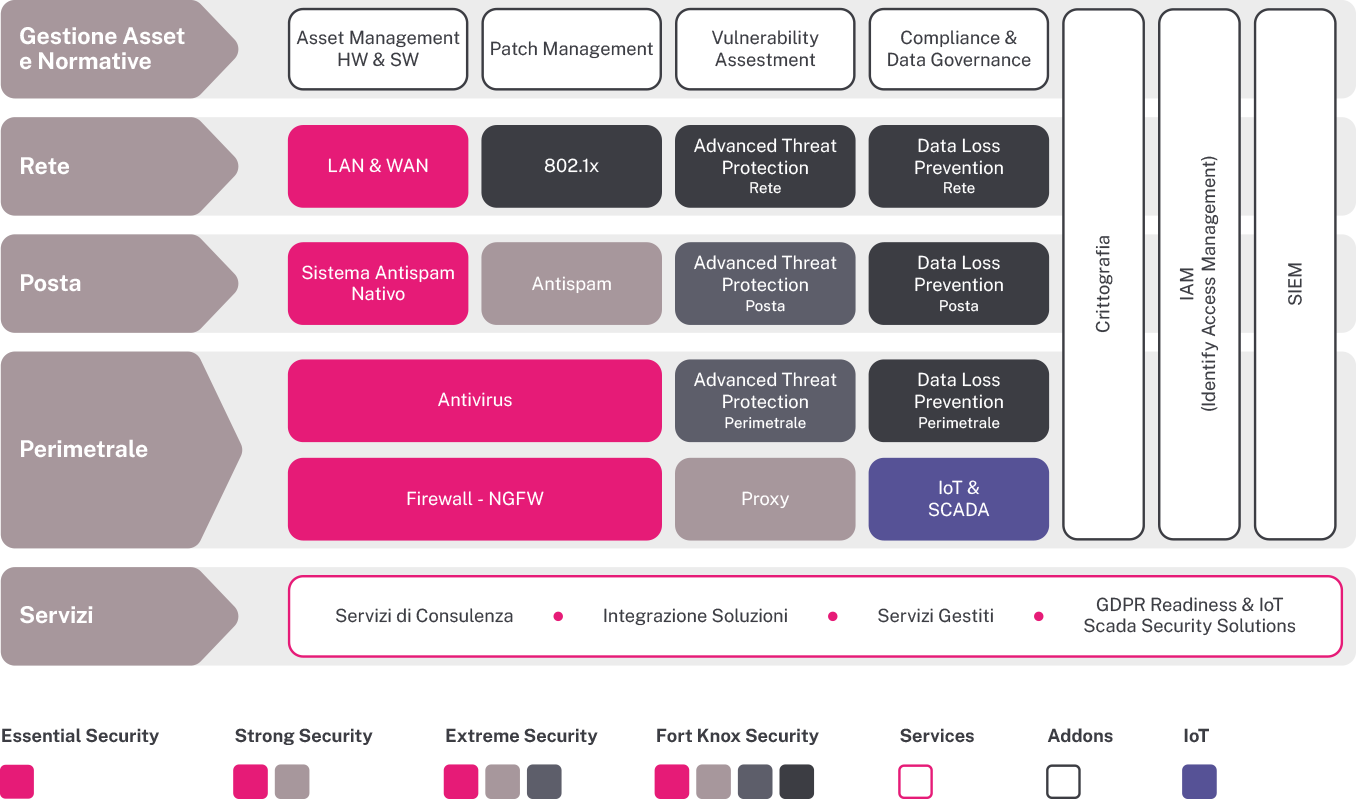
\includegraphics[width=0.9\linewidth]{images/wtc/sec-matrix.png}
    \caption{Matrice della Sicurezza in Wintech}
    \label{fig:sec-matrix}
\end{figure}

\section{Partnership e Certificazioni}

Come supporto a tutto il proprio lavoro, Wintech ha dalla sua parte una serie di \emph{partnership} con produttori e fornitori degli strumenti che poi utilizza. Tra questi troviamo aziende come \emph{HPE Aruba}, \emph{Cambium Networks}, \emph{PaloAlto Networks} e \emph{Watchguard} per il lato \emph{network} e altre come \emph{Nutanix}, \emph{Veeam} e \emph{WMware} per la parte di infrastruttura e virtualizzazione.\cite{site:wtc-dati} Inoltre mantiene un rapporto abbastanza diretto tra se e le aziende con cui collabora come \emph{Grandstream} e \emph{Sangfor}, la seconda oggetto del mio progetto di stage.

\begin{figure}[htbp]
    \centering
    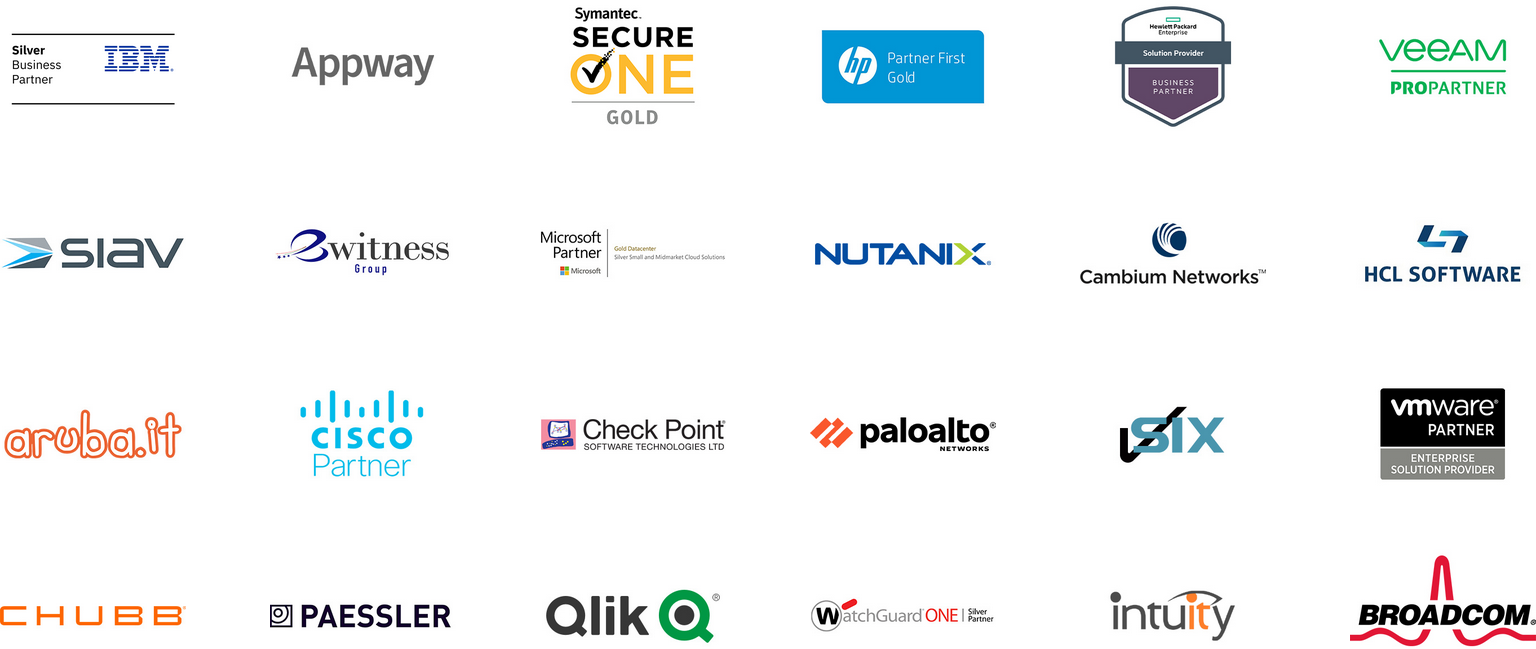
\includegraphics[width=0.8\linewidth]{images/wtc/partner.png}
    \caption{Loghi dei partner di Wintech}
    \label{fig:partner-wtc}
\end{figure}

Dal lato delle certificazioni invece, l'azienda è certificata rispetto agli standard \textbf{UNI CEI ISO/IEC 9001:2015} e \textbf{UNI CEI ISO/IEC 27001:2017}. La prima attesta la qualità per le attività di progettazione, implementazione e fornitura di sistemi informativi integrati, progettazione e sviluppo di soluzioni software e erogazione di assistenza tecnica, sistematica e applicativa.

La seconda invece assicura che i servizi sistemistici e di \emph{network} forniti in \emph{outsourcing} garantiscano \textbf{riservatezza} rispetto agli accessi alle informazioni e \textbf{integrità} e \textbf{disponibilità} di queste ultime.

\begin{figure}[htbp]
    \centering
    \begin{subfigure}[b]{0.4\linewidth}
        \centering
        
\includegraphics[width=0.8\linewidth]{images/wtc/ISO-9001.png}
        \caption{Certificazione ISO 9001}
        \label{fig:iso-9001}
    \end{subfigure}
    \hfill
    \begin{subfigure}[b]{0.4\linewidth}
        \centering
        
\includegraphics[width=0.8\linewidth]{images/wtc/ISO-27001.png}
        \caption{Certificazione ISO 27001}
        \label{fig:iso-27001}
    \end{subfigure}
    \caption{Certificazioni ISO di Wintech}
    \label{fig:iso-wtc}
\end{figure}

\section{Organizzazione interna}

Wintech suddivide le risorse in modo che vi sia una struttura che permetta a figure tecniche e specializzate di lavorare su ambiti ben definiti ed attività elementari. L'organizzazione è divisa in varie divisioni tra cui \textbf{\emph{Marketing}}, \textbf{Commerciale}, \textbf{Sviluppo} e \textbf{Sistemi}, con ovviamente i reparti di \textbf{Risorse Umane} e \textbf{Direzione}. Si possono trovare inoltre gruppi di \textbf{Ricerca e Sviluppo} e quelli di \textbf{Help Desk}. Ogni unità operativa è gestita da un proprio responsabile, un \textbf{\emph{Project Manager}}.

\section{Tecnologie aziendali}
Tutta l'azienda si basa su tecnologie di grado \emph{enterprise}, sfruttando principalmente l'ecosistema offerto da Microsoft, ma anche con altri strumenti \emph{open-source}, talvolta gratuiti.

La maggior parte dei dispositivi aziendali utilizza come sistema operativo \emph{Windows 11}, altri \emph{Windows 10} e molti server usano varie versioni di \emph{Windows Server}. Tuttavia sono presenti alcuni dispositivi Apple che montano \emph{MacOS} e alcuni server che operano su sistemi \emph{Linux} delle famiglie \emph{Debian} e \emph{RedHat}, ad esempio \emph{CentOS}.

Per la gestione documentale si affida a \emph{Microsoft Office 365}, mentre per le comunicazioni vengono utilizzati \emph{Microsoft Outlook} per la gestione delle \emph{mail} e \emph{Microsoft Teams} per la messaggistica istantanea e chiamate video e non.

Gli strumenti utilizzati all'interno dell'infrastruttura di rete e per la sicurezza aziendale verranno trattati nel \autoref{cap:tecnologie}, in quanto parte integrante della formazione iniziale del percorso di stage.

\section{Propensione all'innovazione}

Come presentato prima nelle sottosezioni \ref{sez:azienda-cloud} e \ref{sez:azienda-security}, Wintech è la prima a proporre soluzioni innovative e all'avanguardia ai propri clienti. La sua capacità di mantenersi aggiornata sulle nuove tecnologie e sfruttando l'esperienza acquisita negli anni, le ha permesso di mantenersi competitiva e rilevante sul mercato.

Tra i vari prodotti offerti e promossi dall'azienda troviamo strumenti per \emph{eLearning}\cite{site:wtc-elearning} e prodotti di \emph{Enterprise Resource Planning} (ERP)\cite{site:wtc-erp}. Due dei punti cardine dei progetti di Wintech sono la \emph{Digital Transformation}\cite{site:wtc-digital} e la \emph{Social Collaboration}\cite{site:wtc-collab}, per sfruttare al meglio le tecnologie digitali ed essere più competitivi sul mercato. Inoltre si cerca di promuovere la comunicazione, la condivisione e la collaborazione tra colleghi, favorendo e aumentando l'\emph{engagement} dei dipendenti e la crescita delle loro competenze, creando un clima confortevole e accogliente all'interno del posto di lavoro.

\begin{figure}[!htbp]
    \centering
    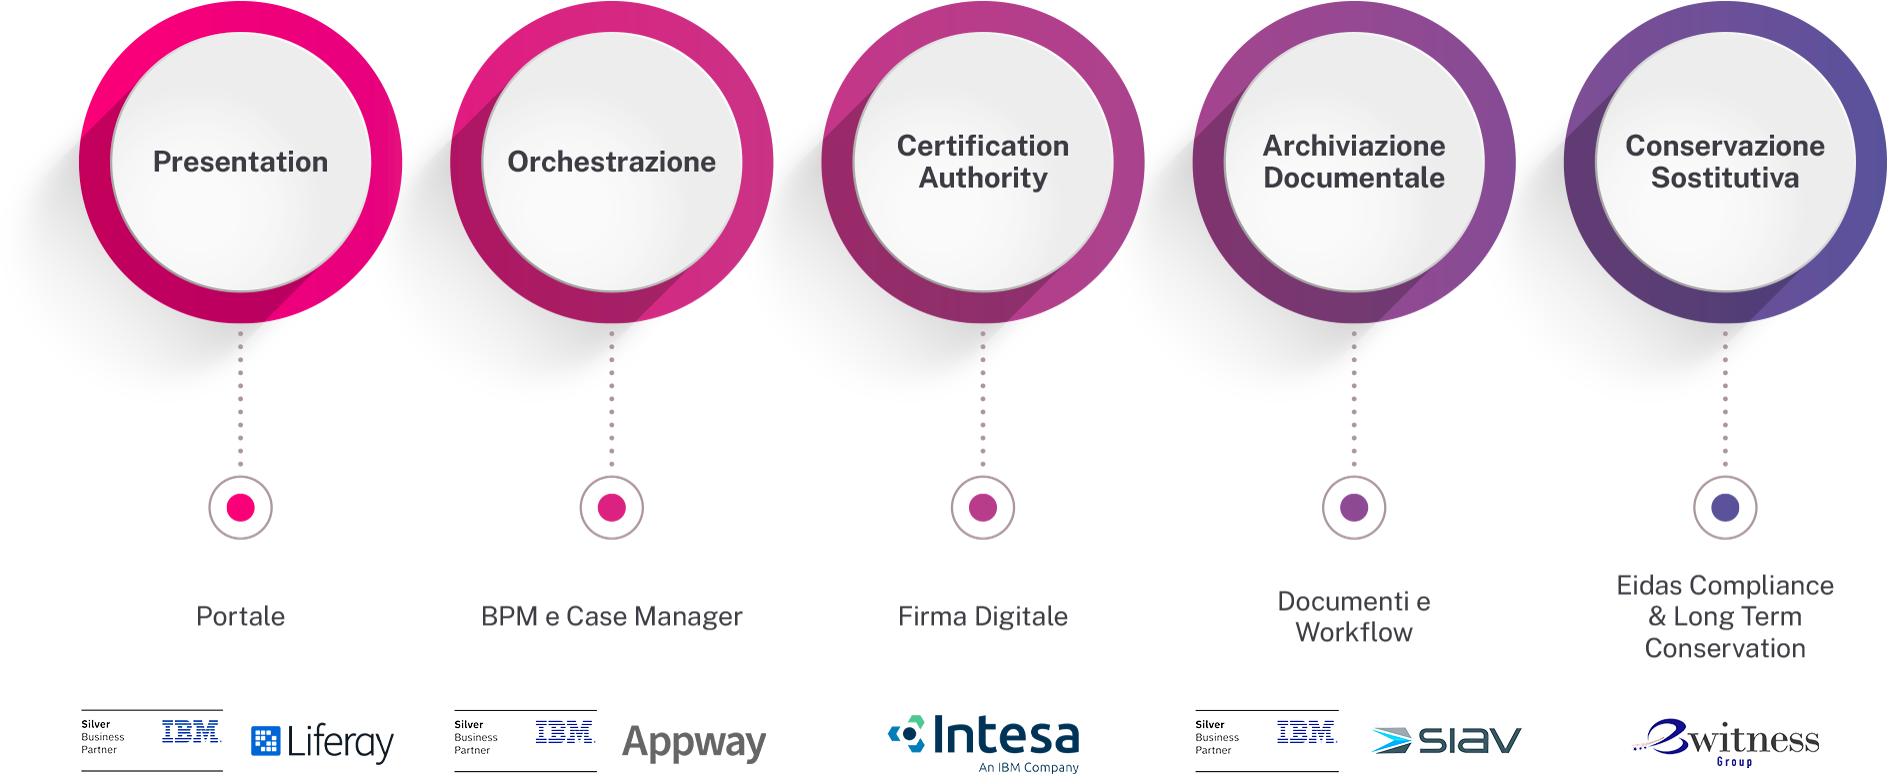
\includegraphics[width=\linewidth]{images/wtc/digital-transform.png}
    \caption{Il progetto di \emph{Digital Transformation} di Wintech}
    \label{fig:digital-transformation}
\end{figure}

\begin{figure}[!htbp]
    \centering
    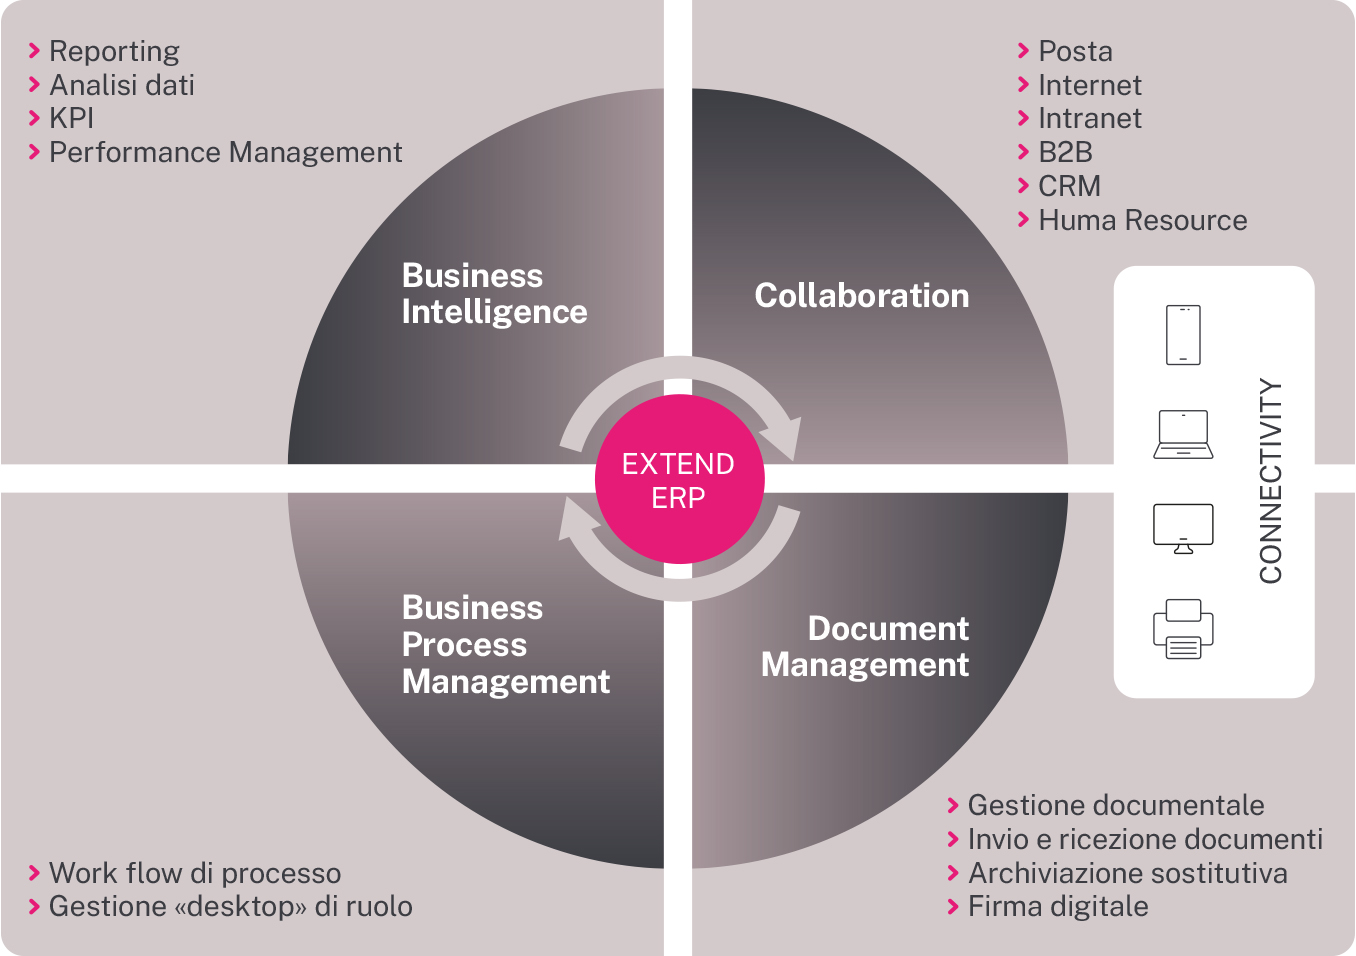
\includegraphics[width=0.8\linewidth]{images/wtc/erp.jpg}
    \caption{Schema di funzionamento di una soluzione \emph{ERP}}
    \label{fig:erp-schema}
\end{figure}

\section{Lo stage nella strategia aziendale}

Il mio primo contatto con l'azienda è avvenuto tramite l'evento Stage-IT. Quest'ultimo è stato promosso da Confindustria Veneto Est con i Dipartimenti di Matematica e Scienze Statistiche dell'Università di Padova e partecipato dal Dipartimento di Ingegneria Informatica per favorire l'incontro tra aziende con progetti innovativi nell'ambito IT e studenti dei corsi di laurea in Informatica, Statistica e Ingegneria Informatica interessati allo svolgimento di tirocini. Wintech partecipa all'evento da diversi anni e ha sempre avuto un buon riscontro, sia da parte degli studenti che da parte delle aziende.

Per lo studente lo stage gioca un ruolo importante nella sua formazione e proprio per questo viene consigliato come ultima fase nel percorso universitario, in quanto permette di applicare le conoscenze, sia teoriche che pratiche, ottenute durante il percorso di studi. Inoltre, l'esperienza avuta con il progetto del corso di Ingegneria del Software mette molti alla prova con la necessità di lavorare in un \emph{team} di più persone da coordinare per consegnare un prodotto ad un committente esterno con la necessità di risolvere un problema reale. Inserire dunque uno studente in un contesto aziendale offre al tirocinante la possibilità di "toccare con mano" quello che è il mondo del lavoro, apprendendo dinamiche e processi interni e permettendo di capire se il percorso intrapreso è quello giusto per lui.

Per un'azienda, invece, lo stage è un'opportunità per valutare le capacità degli studenti nel realizzare prodotti con uno scopo pratico e ben definito, non usa e getta. Spesso l'esperienza di stage viene utilizzata anche come strumento per conoscere nuove persone da inserire in organico e non solo ospitando uno studente per due mesi da utilizzare come manodopera a basso costo, ma bensì come un'opportunità per confrontarsi con qualcuno con conoscenze aggiornate e che può portare nuove idee e punti di vista, con un ottica di miglioramento continuo e a lungo termine.

Wintech sotto questo punto di vista propone progetti legati a prodotti che verranno o sono già utilizzati internamente o dai propri clienti. Proprio per questo cerca di instaurare un rapporto con lo stagista fin da subito basato su rispetto e fiducia e verrà considerato da tutti i dipendenti come un collega a tutti gli effetti. Questo, oltre a fornire un ambiente stimolante e confortevole, responsabilizza il tirocinante a lavorare al meglio per non creare problemi agli altri \emph{team} durante lo sviluppo del proprio progetto.

Per una buona riuscita dello stage è necessario anche un buon rapporto e dialogo tra tutor e stagista. In Wintech si è seguiti e formati con attenzione all'inizio del percorso, in modo da rendersi poi autonomi e riferire in caso di necessità. Questo non significa essere lasciati a se stessi dopo poco, anzi tutti i componenti del \emph{team} in cui si viene inseriti (e non solo) sono disponibili a rispondere a qualsiasi domanda, anche su argomenti non strettamente legati al progetto, e a confrontarsi in caso di problemi o possibili migliorie e soluzioni alternative.

\section{Scelta dell'azienda}

All'evento StageIT tutte le aziende partecipanti esponevano brevemente i progetti che proponevano. Questo mi ha permesso preventivamente di scegliere quelle che più mi interessavano, senza limitare la mia ricerca. Durante tutto il pomeriggio passato nel padiglione della fiera ho cercato di parlare con più aziende possibili, in modo da capire meglio cosa offrissero e quali fossero le loro aspettative, ma anche scoprire progetti non pubblicizzati, essendo le proposte limitate ad un numero massimo di tre.

La maggior parte dei partecipanti erano propositivi e interessati ad avere un colloquio con gli studenti, per capire al meglio le loro capacità e le loro aspettative. Come esperienza mi ha permesso di avere molte piccoli brevi colloqui con responsabili aziendali, grazie ai quali sono riuscito a capire meglio cosa cercare in un'azienda e cosa offrire.

Dopo l'evento ho ricevuto diverse proposte sia da parte di aziende che avevo visitato sia dalle altre, ma dopo l'incontro in sede Wintech per discutere del progetto, ho scelto quest'ultima per la possibilità di lavorare su un campo che mi interessava e diverso da tutte le altre offerte legate principalmente allo sviluppo \textit{software}. Questo mi ha permesso di avere un contatto diretto con il mondo del lavoro, in particolare in un settore che avevo visto solo superficialmente in precedenza durante i periodi di alternanza scuola-lavoro in aziende che offrivano servizi e consulenza in ambito \textit{networking}.